\documentclass[12pt]{article}
\usepackage{amsmath}
\usepackage{graphicx}
\usepackage{hyperref}
\usepackage{listings}
\usepackage{color}
\usepackage{pythonhighlight}

\title{Operating System Course Report - First Half of the Semester}
\author{A class}
\date{\today}

\begin{document}

\maketitle
\newpage

\tableofcontents
\newpage

\section{Introduction}
This report summarizes the topics covered during the first half of the Operating System course. It includes theoretical concepts, practical implementations, and assignments. The course focuses on the fundamentals of operating systems, including system architecture, process management, CPU scheduling, and deadlock handling.

\section{Course Overview}
\subsection{Objectives}
The main objectives of this course are:
\begin{itemize}
    \item To understand the basic components and architecture of a computer system.
    \item To learn process management, scheduling, and inter-process communication.
    \item To explore file systems, input/output management, and virtualization.
    \item To study the prevention and handling of deadlocks in operating systems.
\end{itemize}

\subsection{Course Structure}
The course is divided into two halves. This report focuses on the first half, which covers:
\begin{itemize}
    \item Basic Concepts and Components of Computer Systems
    \item System Performance and Metrics
    \item System Architecture of Computer Systems
    \item Process Description and Control
    \item Scheduling Algorithms
    \item Process Creation and Termination
    \item Introduction to Threads
    \item File Systems
    \item Input and Output Management
    \item Deadlock Introduction and Prevention
    \item User Interface Management
    \item Virtualization in Operating Systems
\end{itemize}

\section{Topics Covered}

\subsection{Basic Concepts and Components of Computer Systems}
This section explains the fundamental components that make up a computer system, including the CPU, memory, storage, and input/output devices.

\subsection{System Performance and Metrics}
This section introduces various system performance metrics used to measure the efficiency of a computer system, including throughput, response time, and utilization.

\subsection{System Architecture of Computer Systems}
Describes the architecture of modern computer systems, focusing on the interaction between hardware and the operating system.

\subsection{Process Description and Control}
Processes are a central concept in operating systems. This section covers:
\begin{itemize}
    \item Process states and state transitions
    \item Process control block (PCB)
    \item Context switching
\end{itemize}

\subsection{Scheduling Algorithms}
This section covers:
\begin{itemize}
    \item First-Come, First-Served (FCFS)
    \item Shortest Job Next (SJN)
    \item Round Robin (RR)
\end{itemize}
It explains how these algorithms are used to allocate CPU time to processes.

\subsection{Process Creation and Termination}
Details how processes are created and terminated by the operating system, including:
\begin{itemize}
    \item Process spawning
    \item Process termination conditions
\end{itemize}

\subsection{Introduction to Threads}
This section introduces the concept of threads and their relation to processes, covering:
\begin{itemize}
    \item Single-threaded vs. multi-threaded processes
    \item Benefits of multithreading
\end{itemize}

\begin{figure}[h]
    \centering
    \includegraphics[width=0.5\textwidth]{/Users/khawaritzmi/Unhas/os_report_mid2024/a_class/asset/example.png}  % Sesuaikan nama file dan ukurannya
    \caption{Ini adalah gambar contoh dari multithreading.}
    \label{fig:contoh_gambar}
\end{figure}

Seperti yang terlihat pada Gambar \ref{fig:contoh_gambar}, inilah cara menambahkan gambar dengan keterangan.

\subsection{File Systems}
File systems provide a way for the operating system to store, retrieve, and manage data. This section explains:
\begin{itemize}
    \item File system structure
    \item File access methods
    \item Directory management
\end{itemize}

\subsection{Input and Output Management}
\subsubsection{\textit{Interfacing Input/Output}}
\textit{Interfacing I/O} adalah peralatan yang digunakan untuk menghubungkan suatu piranti dengan CPU melalui \textit{bus}. Tujuannya adalah mengontrol dan mentransfer data antara perangkat I/O dan CPU/memori melalui \textit{bus} dan \textit{controller}.
Komponen \textit{Interfacing I/O}:
\begin{itemize}
    \item Perangkat I/O: \textit{keyboard, mouse, monitor, printer,} dll.
    \item I/O \textit{Controller}: Perangkat keras yang mengontrol dan mengelola komunikasi antara 
    \item \textit{Bus}: Jalur komunikasi data antara perangkat I/O dan sistem komputer.
    \item \textit{Driver Software}: Perangkat lunak yang memungkinkan sistem operasi mengenali dan mengontrol perangkat I/O.
\end{itemize}

\subsubsection{Sistem Prosesor}
\begin{enumerate}
    \item {Saluran I/O}
Merupakan sebuah prosesor khusus dengan kemampuan terbatas yang disusun untuk interface beberapa piranti I/O ke memori. Saluran I/O dapat melakukan pendeteksian dan pembetulan kesaIahan dan beroperasi dalam basis \textit{cycle stealing}. Saluran I/O berkomunikasi dengan CPU sebagai suatu fasiIitas DMA dan berkomunikasi dengan piranti I/O seolah¬-olah sebuah CPU. Karena piranti I/O mempunyai kecepatan transfer yang berbeda-beda, maka saluran dibagi menjadi 3 pelayanan, yaitu:
\begin{enumerate}
    \item Saluran \textit{Multiplexer} \\
    Digunakan untuk menghubungkan piranti yang berkecepatan rendah dan sedang serta mengoperasikannya secara bersamaan dengan \textit{multiplexing}.
    \item  Saluran \textit{Selector} \\
    Digunakan untuk menghubungkan piranti I/O yang berkecepatan tinggi tanpa \textit{multiplexing}. Contoh: pita magnetis, \textit{disk}.
    \item Saluran \textit{Multiplexer} Blok \\
    Merupakan kombinasi dari dua pelayanan diatas.
\end{enumerate}
\end{enumerate}


\subsubsection{Prosesor I/O}
Merupakan komputer umum yang berkomunikasi dengan memori utama melalui fasilitas DMA system bus dan dengan piranti I/O atas satu atau lebih bus I/O.
Ada 2 mode yaitu:
\begin{enumerate}
    \item \textit{Single Shared bus} \\
    Setiap IOP mengendalikan sejumlah piranti I/O tertentu yang tetap.
\begin{figure}[h]
    \centering
    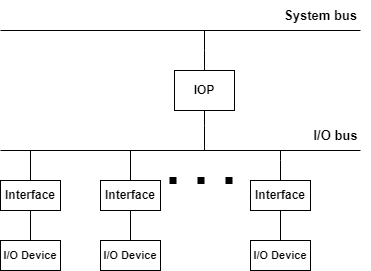
\includegraphics[width=0.5\textwidth]{/asset/Single.png}  % Sesuaikan nama file dan ukurannya
    \caption{Single Matrix bus}
    \label{fig:contoh_gambar}
\end{figure}
    \item \textit{Switching Matriks bus} \\
    Setiap IOP mengendalikan satu piranti I/O
    \begin{figure}[h]
    \centering
    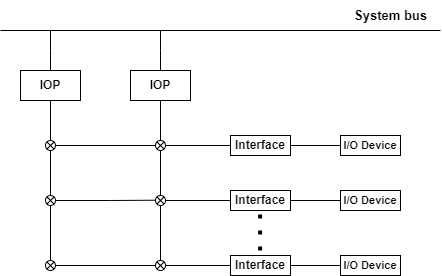
\includegraphics[width=0.5\textwidth]{/asset/Switching.png}  % Sesuaikan nama file dan ukurannya
    \caption{Switching Matriks bus}
    \label{fig:contoh_gambar}
\end{figure}
    \item Konfigurasi \textit{Multiprosesor} \\
    Di dalam satu komputer seakan-akan terdapat beberapa \textit{mikroprosesor}, meskipun sebenarnya \textit{mikroprosesor} utamanya hanya satu, sedangkan yang Iainnya berupa prosesor I/O (lOP). Hubungan yang paling sederhana menggunakan \textit{common bus}.
    \begin{figure}[h]
    \centering
    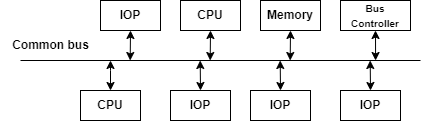
\includegraphics[width=0.5\textwidth]{/asset/Konfigurasi.png}  % Sesuaikan nama file dan ukurannya
    \caption{Ini adalah gambar contoh dari multithreading.}
    \label{fig:contoh_gambar}
\end{figure}
    \begin{itemize}
    \item \textit{Bus} umum bersifat membagi waktu (\textit{time shared}) oleh semua prosesor dan hanya satu prosesor yang dapat mengakses memori pada waktu tertentu.Tetapi dapat juga menggunakan \textit{bus} umum ke dalam organisasi \textit{multiprosesor dual bus}.
    \item Setiap komputer dihubungkan suatu pengendali sistem ke \textit{bus} umum.
    \item Komunikasi interkomputer ini dilakukan pada sistem \textit{bus} melalui memori umum.
\end{itemize}
\begin{figure}[h]
    \centering
    \includegraphics[width=0.5\textwidth]{/asset/systemBus.png}  % Sesuaikan nama file dan ukurannya
    \caption{System bus}
    \label{fig:contoh_gambar}
\end{figure}
\end{enumerate}
Input and output management is key for handling the interaction between the system and external devices. This section includes:
\begin{itemize}
    \item Device drivers
    \item I/O scheduling
\end{itemize}

\subsection{Deadlock Introduction and Prevention}
Explores the concept of deadlocks and methods for preventing them:
\begin{itemize}
    \item Deadlock conditions
    \item Deadlock prevention techniques
\end{itemize}

\subsection{User Interface Management}
This section discusses the role of the operating system in managing the user interface. Topics covered include:
\begin{itemize}
    \item Graphical User Interface (GUI)
    \item Command-Line Interface (CLI)
    \item Interaction between the user and the operating system
\end{itemize}

\subsection{Virtualization in Operating Systems}
Virtualization allows multiple operating systems to run concurrently on a single physical machine. This section explores:
\begin{itemize}
    \item Concept of virtualization
    \item Hypervisors and their types
    \item Benefits of virtualization in modern computing
\end{itemize}

\section{Assignments and Practical Work}
\subsection{Assignment 1: Process Scheduling}
Students were tasked with implementing various process scheduling algorithms (e.g., FCFS, SJN, and RR) and comparing their performance under different conditions.
\subsubsection{Group 1}
\begin{python}
    class Process:
    def __init__(self, pid, arrival_time, burst_time):
        self.pid = pid
        self.arrival_time = arrival_time
        self.burst_time = burst_time
        self.completion_time = 0
        self.turnaround_time = 0
        self.waiting_time = 0
\end{python}

\begin{table}[htbp] % Optional: For floating position
    \centering
    \begin{tabular}{|c|c|c|} % Defines number of columns and alignment (c = center, l = left, r = right). '|' creates vertical lines.
    \hline
    Header 1 & Header 2 & Header 3 \\ % Column headers
    \hline
    Row 1, Column 1 & Row 1, Column 2 & Row 1, Column 3 \\ % First row of data
    \hline
    Row 2, Column 1 & Row 2, Column 2 & Row 2, Column 3 \\ % Second row of data
    \hline
    \end{tabular}
    \caption{Your table caption} % Optional: For adding a caption
    \label{tab:your_label} % Optional: For cross-referencing the table
\end{table}
\subsection{Assignment 2: Deadlock Handling}
In this assignment, students were asked to simulate different deadlock scenarios and explore various prevention methods.

\subsection{Assignment 3: Multithreading and Amdahl's Law}
This assignment involved designing a multithreading scenario to solve a computationally intensive problem. Students then applied **Amdahl's Law** to calculate the theoretical speedup of the program as the number of threads increased.
\subsubsection{Group: 9}
Pertanyaan:
Misalkan sebuah program terdiri dari 80\% bagian yang dapat diparalelisasi, sedangkan 20\% tidak dapat diparalelisasi. Berdasarkan Hukum Amdahl, hitung percepatan teoritis yang dapat dicapai jika program tersebut dijalankan dengan 2, 4, 8, dan 16 threads. Tentukan juga batas atas percepatan teoritis saat jumlah threads mendekati tak terbatas.

Gunakan rumus berikut untuk menghitung percepatan teoritis:

\[
S(N) = \frac{1}{(1 - P) + \frac{P}{N}}
\]

Ket:
\begin{itemize}
    \item \( S(N) \) adalah percepatan teoritis dengan \( N \) threads,
    \item \( P \) adalah bagian program yang dapat diparalelisasi,
    \item \( N \) adalah jumlah threads.
\end{itemize}

\begin{python}
    # Menghitung percepatan teoritis menggunakan Hukum Amdahl
def amdahl_law(P, N):
    return 1 / ((1 - P) + (P / N))

# Persentase bagian program yang dapat diparalelisasi
P = 0.80  # 80%

# Daftar jumlah thread yang digunakan
threads = [2, 4, 8, 16, float('inf')]

# Menghitung dan menampilkan percepatan untuk setiap jumlah thread
for N in threads:
    speedup = amdahl_law(P, N)
    print(f"Percepatan teoritis dengan {int(N) if N != float('inf') else 'tak terbatas'} threads: {speedup:.2f}")
\end{python}

\textbf{Penjelasan Output:}

Setelah menjalankan kode di atas, berikut adalah hasil percepatan teoritis (\(S(N)\)) untuk berbagai jumlah threads:

\begin{itemize}
    \item Percepatan dengan 2 threads: 1.33
    \item Percepatan dengan 4 threads: 1.60
    \item Percepatan dengan 8 threads: 1.78
    \item Percepatan dengan 16 threads: 1.88
    \item Percepatan dengan jumlah threads yang tak terbatas: 2.00
\end{itemize}

Hasil ini menunjukkan bahwa seiring bertambahnya jumlah threads, percepatan teoritis meningkat, tetapi tidak secara linear. Sesuai dengan Hukum Amdahl, percepatan maksimal dibatasi oleh bagian dari program yang tidak dapat diparalelisasi. Pada contoh ini, batas atas percepatan adalah 2.0, yang tercapai saat jumlah threads mendekati tak terbatas. Hal ini disebabkan oleh 20\% dari program yang tidak bisa diparalelisasi.

\subsection{Assignment 4: Simple Command-Line Interface (CLI) for User Interface Management}
Students were tasked with creating a simple **CLI** for user interface management. The CLI should support basic commands such as file manipulation (creating, listing, and deleting files), process management, and system status reporting.

\subsection{Assignment 5: File System Access}
In this assignment, students implemented file system access routines, including:
\begin{itemize}
    \item File creation and deletion
    \item Reading from and writing to files
    \item Navigating directories and managing file permissions
\end{itemize}

\section{Conclusion}
The first half of the course introduced core operating system concepts, including process management, scheduling, multithreading, and file system access. These topics provided a foundation for more advanced topics to be covered in the second half of the course.

\end{document}
